% !TEX program = xelatex
\documentclass[a4paper,12pt, oneside]{article}
\usepackage[utf8]{inputenc}

\usepackage{graphicx} % To include images
\usepackage{xcolor} % To have more colors and be able to define new one
\usepackage{afterpage} % For the page background color
\usepackage{listings} % To include code snippets
\usepackage{indentfirst} % To indent the first paragraph
\usepackage{url} % For url...
\usepackage[all]{nowidow} % To prevent widow/orphan lines
\usepackage[margin=2.5cm]{geometry} % To change the margin
\usepackage[justification=justified,singlelinecheck=false]{caption} % To left align even the single line captions
\usepackage{multicol} % Enable multi columns environment
\usepackage{subcaption} % To have two figures next to each other
\usepackage{fontspec} % For custom fonts
\usepackage{lipsum} % Lorem ipsum generator
\usepackage{layouts} %to get the text width in cm
\usepackage{rotating} %to have some figures sideways.
\usepackage{placeins} % To force floats to be placed before the beginning of next section
\usepackage{parskip} % To add space between paragraphs

\usepackage{tikz}
\usepackage{pgf-umlsd}
\usepgflibrary{arrows}
\usetikzlibrary{positioning,fit,calc}

\setmainfont{Graublau Sans}
\setlength{\parindent}{1.5em}

\definecolor{gray}{rgb}{0.4,0.4,0.4}
\definecolor{darkblue}{rgb}{0.0,0.0,0.6}
\definecolor{cyan}{rgb}{0.0,0.6,0.6}
\definecolor{rocketorange}{rgb}{1,.4,0}

% Customized commands
\newcommand{\HRule}{\rule{\linewidth}{0.5mm}}

\DeclareUrlCommand\email{\urlstyle{rm}}

%Acknowledgements environment
\newenvironment{acknowledgments}
  {\renewcommand{\abstractname}{Acknowledgments}
   \begin{abstract}}
  {\end{abstract}}

\begin{document}
\pagenumbering{roman}

% !TEX root = main.tex
%\pagecolor{rocketorange}
%\color{white}

\begin{titlepage}

\begin{center}

% Upper part of the page
\begin{minipage}{6in}
  \centering
  $\vcenter{\hbox{\includegraphics[width=55mm]{logos/logo_EPFL.pdf}}}$
  \hspace*{2cm}
  $\vcenter{\hbox{
\includegraphics[width=55mm]{logos/NothingInteractive_RGB_Color_Vertical.pdf}}}$
\end{minipage}\\[2 cm]

{\large School of Computer and Communication Sciences IC}\\[0.5cm]
{\large Computer Science Section}\\[0.5cm]
{\Large Master Thesis Project}\\[0.5cm]


% Title
%\HRule
\vspace{1cm}
{\huge \bfseries Flok: Collaboratively solve problems through participatory design thinking}\\[0.4cm]

%\HRule
\vspace{1.5cm}

\large \emph{Author:} David \textsc{Sandoz}\\[1.5cm]

% Supervisors
\begin{minipage}{0.5\textwidth}
\begin{flushleft} \large
\emph{EPFL Supervisor:}\\
Prof. Denis \textsc{Gillet}\\
Coordination \& Interaction Systems Group REACT
\end{flushleft}
\end{minipage}
\begin{minipage}{0.4\textwidth}
\begin{flushright} \large
\emph{Company Supervisor:}\\
Bastiaan \textsc{van Rooden}\\
Nothing GmbH\\
~
\end{flushright}
\end{minipage}

\vfill

% Bottom of the page
{\large March 2016}

\end{center}

\end{titlepage}

\pagecolor{white}
\color{black}


\vspace*{5cm}
\begin{acknowledgments}
    \lipsum[1] %TODO
\end{acknowledgments}
\vfill
\textbf{Author/student's contact details}\\
David \textsc{Sandoz}\\
Les Allées 29\\
2300 La Chaux-de-Fonds\\

\noindent
\email{contact@davidsandoz.ch}
\newpage

\vspace*{5cm}
\begin{abstract}
    Humans have ideas and they are generally improved when those are shared and discussed among several people.
    However, it can get quite messy and our goal is to design and develop a platform – Flok – that significantly improves collaboration around ideas, while providing an experience as human as possible.
    To do so, we take a user-centered approach by using processes such as the creation of personas, user story mapping, wireframing and prototyping.
    Based on those processes and a well defined information architecture, we build a front-end application.
    The back-end is not implemented but has an important role in order to have a final fully working product.
    It is not implemented because we choose to prioritize user testing.
    We are able to improve the front-end and verify some of our assumptions by doing three test sessions.
    This is a bit weak to make strong conclusions, but the feedback we get is promising and tells us we are going in the right direction.
    Building the back-end is one of the important next steps that will allow us to have a fully working application.
    Combining that with more user testing will allow us to validate or invalidate further assumptions.
\end{abstract}
\newpage

\tableofcontents
\newpage

\setcounter{page}{1}
\pagenumbering{arabic}

% Text width in cm: \printinunitsof{cm}\prntlen{\textwidth}

\section{Introduction}
Humans have ideas. Not a lot of those ideas end up being applied, no matter if they are good or bad.
Sometimes they just stay in the head of the person who had one and are not developed further because the person thinks it is not a good idea.
She might be right but she can't really know as long as she has not shared her idea.
And of course it happens that people do share their ideas.
That is something good to do because it can bring a lot of valuable input that we do not necessarily think about by ourselves.
This makes the idea evolve; it might go in one direction or another, change shape, or even generate new different ideas.
This can also be seen as what is called \emph{brainstorming}. This process is in general quite messy.
A lot of information is generated and not structured, which makes it difficult to highlight the most important items.
For brainstorming, teams sometimes use a ticketing system that they already use for other projects related tasks.
Tickets are great for development, but not good for creative brainstorming.

Therefore, what we want to achieve is to design and develop a platform that significantly improves collaboration around ideas within a team or a small to medium-sized company by getting considerably close to the cognitive working reality of a team.
We want to have a more human experience.
This will enable the users to have an effective way to bubble up the good ideas among all the information, and also to drive the sharing of new ideas.
All this should be highly intuitive and straightforward to use, by being particularly careful about the overall user experience of the platform.

\subsection{Flok}
Flok is the name of the platform we want to build.
This name comes from the term \emph{flock}, representing a large number of entities – people – moving together.
It fits well as we really want to focus on the collaboration among a group of people and how, together, they make ideas evolve, while respecting human behavior.

\subsection{Hypothesis}
\label{hypothesis}
It can be proven that a truly real-time approach to create, read and update information within on-site or remote, (inter-)disciplinary teams significantly improves their shared know-how and overall collaborative spirit thus leading to a verifiable increase of their creative potential.

\subsection{User-centered design}
The approach taken to create the platform is based on the \emph{user-centered design} concept.
The goal is to focus first on the user need and to start by designing the user interaction with the product to then define what the content is going to be and which technologies are going to be used.
The reason why we took this approach is because we really want the product to be intuitive for the end-users, that it matches their expectations regarding what they need, what they can do with the platform, rather than making them adapt their behavior.

To this end, different processes were used, such as \emph{User Story Mapping} to define the user needs, \emph{Wireframing} and \emph{Prototyping} to quickly test if the design of a functionality matches those user needs, and \emph{User testing} to have feedback from real users in order to adapt the platform to their expectations.
Moreover, we are not going through these different processes sequentially, but rather iteratively.
Each of these steps enable us to discover new issues, new opportunities and we have then to reflect those in every step.

% TODO What about integrating the "Product Design Process" of Nothing Interactive?
% Answer: Not necessarily. It is quite complex to explain, what is already in this section might be enough

\section{Personas}
In order to embrace the user-centered design concept, we have to put ourselves in the shoes of the users we expect to use the platform. To do this, \emph{personas} were created.
They are behavioural patterns build up from the ground who represent the different type of users that we might have.
We made three of them for the project.
All three work in the same startup. \emph{Andrew McAllister} is the CEO, \emph{Melanie Carter} a developer, and \emph{Sergei Fleming} an interaction designer.
These personas were not defined in much more details, as part of the research was to determine more clearly for which purpose Flok is going to be used.

\section{User Story Mapping}
\emph{User Story Mapping} (USM) is a technique which help teams developing software to stay focused on users and their needs \cite{patton2014user}.
It is based on user stories and story maps. \emph{User stories} are descriptions of how users are interacting with the whole product and not only with one of its feature. \emph{Story maps} are a two-dimensional visual representation of stories with \emph{cards} as atomic parts.
In general, the top row of cards represents the backbone of the story (from left to right), and the cards below give more details.
In addition to the focus it gives on the users, USM enables the discussion within the team who builds it to create a shared understanding of the product.
User story maps can be done with software tools which make it easier to edit and share. However, team collaboration is enhanced when people are facing a physical user story map made of sticky notes, which is what has been done for this project.

The user story map constantly evolves throughout the development of the project.
In figure \ref{fig.flokUsmEvolution} you have an overview of how it evolved for Flok.
Figure \ref{fig.flokUsmCurrent} shows you its state at the time of handing in this report.

The green sticky notes represent actions by users and the blue ones indicate which user are doing the actions.
In the latest versions of the user story map, we can notice that the orange sticky notes entitle \emph{slices}, of the story.
As said, the first row is the backbone.
Below we have three slices R1, R2 and R3, \emph{R} meaning \emph{release}.
It helps to define clearly which part of the story are the most important and therefore need to be possible to do for the user in the earliest versions of Flok. For the Master project, we went implemented the front-end up to R2 and left in R3 parts of the stories we did not deem necessary to have in an early version of Flok.

Building this user story map was a bit more tricky than it can be for most others.
Indeed, as Flok interest resides in the real-time interactions between its users, the story has to jump often from a user to another.
This makes it also more difficult to follow when reading the story map.

\begin{figure}[!htb]
    \centering
    \includegraphics[width=\textwidth]{images/flokUsmEvolution.png}
    \caption{Evolution of the user story map for Flok}
    \label{fig.flokUsmEvolution}
\end{figure}

\begin{figure}[!htb]
    \centering
    \includegraphics[width=\textwidth]{images/flokUsmCurrent.jpg}
    \caption{Current state of the user story map for Flok}
    \label{fig.flokUsmCurrent}
\end{figure}

\FloatBarrier
\subsubsection*{Story description}
The story simply start with Andrew having a rough idea that he wants to share in order to discuss about it and develop it.
He then adds the idea on Flok and describe it with text, but images as well.
From here, other users can take part to the idea. For instance, Melanie is looking for interesting ideas in the \emph{discovery} section of the app and she get inspired by the one from Andrew.
From here, she has several possibilities.
She can simply bookmark the idea in order to have it saved and hence, easily come back to it later.
She can also follow the idea in order to get informed of the activity occurring within it.
Then, as she is interested, she goes through a page which recaps the discussion around the idea.
This helps her to quickly have a good overview.
If she wants to actively take part to the idea, she can go to the discussion section and read the last comments before interacting.
As it happens, she agrees with Andrew's comment and show it by \emph{liking} it and replying directly to it.
Moreover she wants to find that comment later so she bookmarks it.
Then she gives her input by writing comments and sharing documents and images.
However, Andrew disagrees with the input from Melanie and he says it by replying to the corresponding comment.

Among the comments and other inputs of team mates taking part to Andrew's idea, he gets interested by the views of one specific person.
He looks at this person profile and more precisely in which other ideas she is active and that might interest him.

Back to Andrew's idea, after a while, Sergei joins the idea that he found through the \emph{discovery} section of the app.
He found the idea interesting and noticed that among the followers there were team mates he usually like their thinking.
He catches up the discussion through the recap and among the highlighted items one image appealed him.
He brings up the image in its context, in the discussion, to see in more details what it is about.
This makes him think about another idea so instead of replying at this point of the discussion, he rather decides to branch from the image to create a new idea in Flok.

Initially new ideas are classified under the \emph{Incubating} label.
This is not the case anymore for Andrew's idea which has evolved and became more mature and precise.
Hence he decides to update the classification to \emph{Need to decide} where the discussion should be more about what are going to be the next step to implement the idea.
Moreover, the original name and description of the idea do not suit its content anymore.
Therefore Andrew updates them accordingly.

After a while, the idea reached the \emph{Open for execution} classification where it got successfully implemented.
At this point the idea can be archived, which is what Andrew does.

% TODO link the story map to the hypothesis.

\section{Information architecture}
To accompany and solidify the project it is important to have a good information architecture.
This helps to have a well defined vocabulary for the different elements making the product, and how they interact with each other.
In our case, we made an \emph{entity-relationship diagram} that you can see in figure \ref{fig.erDiagram}.
In the rectangle are the different entities in Flok.
The ovals their attributes and the diamonds are actions representing the relation between entities.
We have to read the relations from top to bottom (e.g. \emph{Persons are actor of Activity items} or \emph{Ideas contain Comments}).
The thickness of the lines and the fact they are an arrow or not also has a specific meaning, described in the bottom right of the figure.
For instance, a person can post none or more comments, but a specific comment is posted by exactly one person.
Also, a comment must be either an image, a file, a system information or a note (a text comment), and any of these four entities has to be a comment.

\begin{sidewaysfigure}[!htb]
    \centering
    \includegraphics[width=\textwidth]{images/erDiagram.pdf}
    \caption{The entity-relationship diagram of Flok, representing its information architecture}
    \label{fig.erDiagram}
\end{sidewaysfigure}

\clearpage

\section{Wireframing}
Once we had a first version of the user story map, the next step was to build wireframes of the user interface.
Wireframes allow to quickly have a very rough view of the components layout and how they fit in the available space.
They enable us to see changes that need to be brought even before we start designing or implementing, and hence save us some precious time.

For instance, initially ideas were called \emph{topics} and when I designed the first wireframes of recap page for a topic, it was a kind of tag cloud with all the ideas discussed in a topic – The most discussed ones being more prominent (see figure \ref{fig.originalRecapWireframes}).
This made us realize two things.
First, there was a lack of shared understanding regarding the scope of the discussions we expect to be held in one topic and therefore also regarding the content of the recap page.
Secondly, the name \emph{topic} was not a good name to describe this concept.
This is what made us change the name for \emph{idea}. It is also more human – Instead of creating a topic on Flok when you have an idea, you just add an idea on Flok when you have one.
This shows that we were able avoid having to change a single line of code to apply this change as it was detected before we start the first prototype.

\begin{figure}[!htb]
    \centering
    \includegraphics[width=\textwidth]{images/originalRecapWireframes.png}
    \caption{Original wireframe design of the recap page. From left to right: the main recap page, the recap page of one idea in the topic, the dialog asking if we want to see an item in its context, an item highlighted in its context.}
    \label{fig.originalRecapWireframes}
\end{figure}

You can notice in the wireframes of figure \ref{fig.originalRecapWireframes} that we choose to represent the app in a mobile screen.
This decision has been made because having less space forces us to think about what is the most important to show to the user.
It is then easier to design a desktop version from the mobile version than the other way around.
The \emph{Mobile First} development is also getting more important as more people are accessing the web from their mobile device before doing so from a desktop computer.

A few other design decisions were taken during wireframing.
For instance, it was initially possible to unlike a comment in a discussion.
This has been removed to only keep the like button.
Indeed, it is not necessary to explicitly express a disagreement with this action which does not bring any constructive feedback and we also want to foster positivity.
A disagreement can still be express with a comment which should be more constructive.

This is also while designing the wireframes that we asked ourselves the question regarding the order the comments in a discussion.
Some researches \cite{mabande2010designing} concluded that having the oldest ones at the top and the more recent ones at the bottom was leading to more engagement from the participant of a discussion.
Following this order is also more human as it follows the natural reading order.
Moreover, as the input field to add comments is at the bottom, having the new comments appearing right above it is also expected.

% TODO link the wireframes to the hypothesis

\section{Prototyping}
The step following wireframing is prototyping.
In this case, the initial goal was to make it mostly visual in order to have a good idea of the look and feel, but also of the possible interactions from the users.
The content would consist of static mock data.
To avoid having to create a full visual design, we decided to use the component library \emph{Material Design Lite}\footnote{\url{http://getmdl.io}}, which is an implementation of \emph{Material Design}\footnote{\url{http://google.com/design/spec}}.
This lightweight library, with the use of some HTML, CSS and simple Javascript, enabled us to quickly have a prototype with a solid visual design (see figure \ref{fig.firstPrototypeScreenshots}).

\begin{figure}[!htb]
    \centering
    \includegraphics[width=\textwidth]{images/firstPrototypeScreenshots.png}
    \caption{Screenshots of Flok first prototype using \emph{Material Design Lite}}
    \label{fig.firstPrototypeScreenshots}
\end{figure}

Improvements and features have been progressively added to the prototype.
With, all the necessary code to keep it interactive.
However, as it was initially planned to be light, having a bigger code base was not adapted with the prototype structure making it quite messy and therefore more difficult to add new components.
The visual result being good, it seemed to be the right moment to start working on the functional front-end of the platform, based on the prototype.

\section{Front-end}
\subsection{Architecture}
\label{sec.architecture}
We wanted the platform to be fully usable from any device.
The easiest way to implement that is to have a responsive web application.
Hence, Javascript and the \emph{MEAN stack} seemed quite appropriate.
These are also technologies in which \emph{Nothing Interactive} has good experience with.
This means that regarding the front-end we went for a single page application made with \emph{AngularJS}.

As we were satisfied with the result of using Material Design for the prototype, we wanted to continue following those guidelines.
Obviously, Material Design Lite was not enough, therefore we had to use another implementation.
Looking at the different alternatives and knowing that we were going to use AngularJS, the decision to use \emph{Angular Material}\footnote{\url{https://material.angularjs.org}} was straightforward.

There are different ways to build an AngularJS application.
Therefore it was important that we clearly define how we were going to structure it.
\emph{Nothing Interactive} has some internal guidelines, but with the arrival of \emph{Angular 2}, it seemed to be a good time to re-think those guidelines in order to write code that would enable an easy transition to this disruptive new version of the framework.
Hence, we made some adaptations based an Angular Style Guide written by John Papa\footnote{\url{https://github.com/johnpapa/angular-styleguide}}, which is endorsed by the Angular team.

Unfortunately, our great focus on building the front-end and having the best user experience possible did not gave us time to build a functional back-end for the app.
At some point we had to take the decision between either building the back-end, or doing the user testing.
The latter seemed more important as it would (in)validate our assumptions regarding the interaction of the user with the platform.
We also estimated that it would bring us valuable feedback to improve the front-end.

Not having a back-end implies some restrictions.
First, it means that once the AngularJS app is loaded in the browser, everything is happening in the browser only and there is no communication with the server, except to get static files such as images.
Therefore, interaction between two users is not possible.
Then, no back-end also means no database and no saved data.
Fortunately, as the front-end is a single page application, as long as the page is not fully refreshed, all the data created by the user while using Flok is saved in memory, including uploaded files.
Therefore the user can still use and evolve in the app.
This is shown in figure \ref{fig.dealingWithoutBackend}, where directives, controllers and service are concepts coming from AngularJS.

\begin{figure}[!htb]
    \centering
    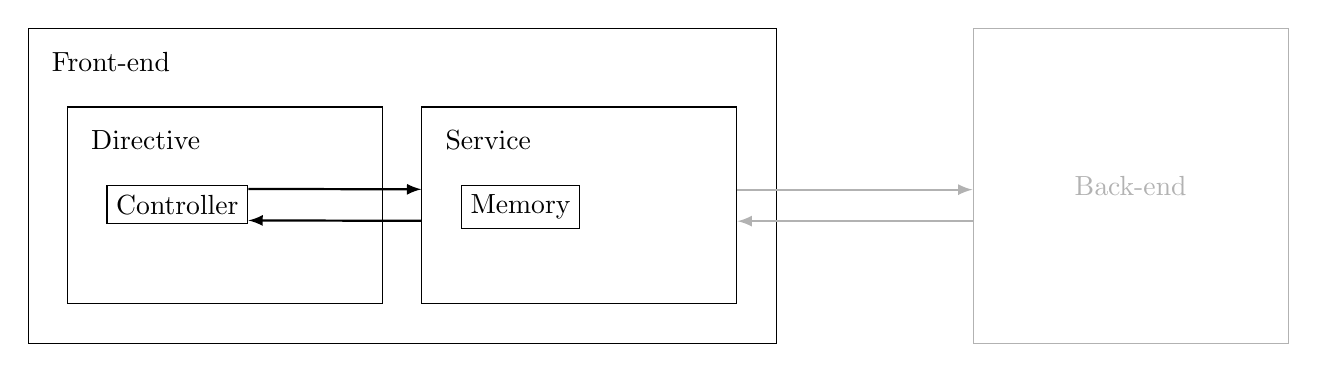
\begin{tikzpicture}
        \node (frontend) [minimum height=4cm, minimum width=9.5cm, draw=black, anchor=north west] at (0,0) {};
        \node [below right, inner sep=.3cm] at (frontend.north west) {Front-end};

        \node (directive) [minimum height=2.5cm, minimum width=4cm, draw=black, anchor=north west] at (.5,-1) {};
        \node [below right, inner sep=.3cm] at (directive.north west) {Directive};

        \node (service) [minimum height=2.5cm, minimum width=4cm, draw=black, anchor=north west] at (5,-1) {};
        \node [below right, inner sep=.3cm] at (service.north west) {Service};

        \node (controller) [draw=black, anchor=north west] at (1, -2) {Controller};
        \node (memory) [draw=black, anchor=north west] at (5.5, -2) {Memory};

        \node (backend) [draw=black!30, color=black!30, minimum height=4cm, minimum width=4cm, anchor=north west] at (12,0) {Back-end};

        \draw[->, >=latex, thick, transform canvas={yshift=2mm}] (controller) -- (service);
        \draw[<-, >=latex, thick, transform canvas={yshift=-2mm}] (controller) -- (service);
        \draw[->, >=latex, thick, transform canvas={yshift=2mm}, color=black!30] (service) -- (service-|backend.west);
        \draw[<-, >=latex, thick, transform canvas={yshift=-2mm}, color=black!30] (service) -- (service-|backend.west);
    \end{tikzpicture}
    \caption{Schema illustrating data flow for Flok. In the front-end, the controllers of directives ask for data to services. Those services should ask the back-end for the information stored in the database. But as there is no back-end, services get the information from their own memory.}
    \label{fig.dealingWithoutBackend}
\end{figure}

We were not trying to build a fully working application without back-end.
Therefore we still kept in mind an architecture that would communicate with a back-end by simulating calls to it, even though we just get the data from memory.

\subsection{Implementation and design decisions}
We are not going to describe the implementation of every component as some of them are quite straightforward.
We are rather going to explain the components where some reflexion had to be made or decisions had to be taken.

\subsubsection{Ideas}
Ideas are the main components of Flok.
They are created by users and they have three different views.
The main view (figure \ref{fig.idea.main}) gives the general information about the idea: author, creation date, description, classification (section \ref{sec.ideasClassification}), followers and relations with other ideas.
From here you can also trigger actions on the idea such as following, bookmarking, archiving and branching (section \ref{sec.branching}).
The available actions depend of the status of the user (creator, follower) toward the idea.
Then there is the discussion view (figure \ref{fig.idea.discussion}) where all the comments (section \ref{sec.comments}) related to the idea can be found.
This is also where comments can be added to the discussion.
Finally there is the recap view (figure \ref{fig.idea.recap} and section \ref{sec.recap}) which highlight the most important comments of the discussion.

\begin{figure}[!htb]
    \begin{subfigure}[t]{.32\textwidth}
        \includegraphics[width=\textwidth]{images/idea.png}
        \caption{Main view}
        \label{fig.idea.main}
    \end{subfigure}
    \hfill
    \begin{subfigure}[t]{.32\textwidth}
        \includegraphics[width=\textwidth]{images/ideaDiscussion.png}
        \caption{Discussion view}
        \label{fig.idea.discussion}
    \end{subfigure}
    \hfill
    \begin{subfigure}[t]{.32\textwidth}
        \includegraphics[width=\textwidth]{images/ideaRecap.png}
        \caption{Recap view}
        \label{fig.idea.recap}
    \end{subfigure}
    \caption{Screenshots of Flok front-end featuring the different views of an idea}
    \label{fig.idea}
\end{figure}

\FloatBarrier
\subsubsection{Ideas classification}
\label{sec.ideasClassification}
Here there is actually not much to say regarding the implementation itself.
We introduced these classification in order to easily visualize the state of an idea.
Initially, to update the classification, it has either to be promoted or demoted, respectively to the next or previous classification.
To do so, one of the idea follower had to start a poll asking all the followers to vote for or against and change of classification (see figure \ref{fig.promotionPoll}).
The goal here was to reflect a common decision.

\begin{figure}[!htb]
    \begin{subfigure}[t]{.32\textwidth}
        \includegraphics[width=\textwidth]{images/promotionPoll_dialog.png}
    \end{subfigure}
    \hfill
    \begin{subfigure}[t]{.32\textwidth}
        \includegraphics[width=\textwidth]{images/promotionPoll_question.png}
    \end{subfigure}
    \hfill
    \begin{subfigure}[t]{.32\textwidth}
        \includegraphics[width=\textwidth]{images/promotionPoll_approved.png}
    \end{subfigure}
    \caption{Screenshots of Flok prototype featuring the promotion poll}
    \label{fig.promotionPoll}
\end{figure}

Then we realized the process can actually get complicated.
What happens if not all followers vote?
Should we wait?
Should we define a time limit to vote? Should such a time limit be define by the poll initiator?
What happens if there is a draw?
We thought about how to reply to these questions and we could have implemented solutions, but in the end this might be a hassle for the user to make that change of state.
Therefore we went for a drastic simplification.
No more poll, no more promotion or demotion.
We simply let any follower update the classification to any available (see figure \ref{fig.classificationSelect}).
The change is instantly applied.
Now there might be disagreement within the followers, but they are all in the same team and they can discuss that.
And as it is so simple to change the classification, they can easily reversed their decisions.
Having simplified this action also enabled us to implement an interactive way for the user to update the classification from desktop, by drag and dropping ideas in \emph{Kanban}\footnote{\url{https://en.wikipedia.org/wiki/Kanban}} columns (see figure \ref{fig.classificationDragAndDrop}).
You will also notice that these columns are color-coded in order to make it even more clearer for the users to understand what can be executed.

\begin{figure}[!htb]
    \null\hfill
    \begin{subfigure}{.32\textwidth}
        \centering
        \includegraphics[width=\textwidth]{images/classificationSelect_selected.png}
    \end{subfigure}
    \hfill
    \begin{subfigure}{.32\textwidth}
        \centering
        \includegraphics[width=\textwidth]{images/classificationSelect_selecting.png}
    \end{subfigure}
    \hfill\null
    \caption{Screenshots of Flok front-end featuring the simple classification update of an idea}
    \label{fig.classificationSelect}
\end{figure}

\begin{figure}[!htb]
    \centering
    \includegraphics[width=\textwidth]{images/classificationDragAndDrop.png}
    \caption{Screenshots of Flok front-end featuring the drag and drop of an idea from a classification to another}
    \label{fig.classificationDragAndDrop}
\end{figure}

\FloatBarrier
\subsubsection{Comments}
\label{sec.comments}
Comments are one of the central components of Flok.
They have one author, they are part of one idea and they are either a note (a text comment), an image, a document, a system information or a deleted comment.
When adding a comment to a discussion, it can be the reply to another comment and thus help to establish relations among comments (see figure \ref{fig.commentView}).
For more details on the properties of each of these type and on the relations of comments with other entities of Flok, we send you back to the entity-relationship diagram in figure \ref{fig.erDiagram}.
We would still like to mention the support of hashtags in comments.
When clicking on one, we are brought to the hashtag view, which list all occurrences of the hashtag in all ideas (see figure \ref{fig.hashtagView}).

Below each comment, a list of actions is offered to the users.
They can like the comment, bookmark it, reply to it or branch it.
Liking a comment helps defining which comments have more value than others.
This will notably be used for the recap view, which we are talking about in section \ref{sec.recap}.
Bookmarking a comment adds it in the bookmark list of the users who can access it from their profile.
It is a way to save comments they want to easily access later.
Comment branching is covered in section \ref{sec.branching}.
And if we are the author of a comment, we have an additional \emph{three dots} button toggling a menu to either edit or delete a comment.

When we introduced the possibility to delete a comment, it was really completely deleted.
However, it also broke relations between comments and ideas, which are made through replies and branches.
Therefore we decided to add the \emph{deleted} comment type, where the content of the comment is deleted, but the object itself not.
Like this the relations are kept.

\begin{figure}[!htb]
    \null\hfill
    \begin{subfigure}[t]{.32\textwidth}
        \centering
        \includegraphics[width=\textwidth]{images/commentView.png}
        \caption{The comment is highlighted, above we have the comment it is replying to and below we have the replies.}
        \label{fig.commentView}
    \end{subfigure}
    \hfill
    \begin{subfigure}[t]{.32\textwidth}
        \centering
        \includegraphics[width=\textwidth]{images/hashtagView.png}
        \caption{The hashtag view list all the occurrences of a hashtag throughout all the ideas.}
        \label{fig.hashtagView}
    \end{subfigure}
    \hfill\null
    \caption{Screenshots of Flok front-end featuring comments and hashtags.}
\end{figure}

\subsubsection{Branching}
\label{sec.branching}
If we try to look at how humans think, they initially have an idea that they brainstorm by themselves or with other people.
It then generates new ideas based on the brainstorm and it can go on until an idea really gets developed and executed.
We tried to represent that in Flok with the \emph{branching} feature.
Basically, you can create an idea by branching another idea or a comment.
The word comes from the software development world, when a copy of source code is made to start developing on it independently.
However it works a bit differently in Flok.
The main goal is to create the relation between the initial idea or comment to the newly created idea.
Nothing is automatically taken from the source which means that the new idea form is blank and the user still has to describe her idea.
Once the idea is created, the discussion can begin, as any new idea.
The difference lies in the relation created, which goals is to represent the human way of thinking.
We wanted to make these relations more visible and therefore implemented visualizations showing branches relations (see figure \ref{fig.branches}).
Clicking on the number of branches from the view of an idea will bring to the idea tree navigation.

\begin{figure}[!htb]
    \null\hfill
    \begin{subfigure}[t]{.32\textwidth}
        \includegraphics[width=\textwidth]{images/branches_idea.png}
        \caption{In the idea view, it is indicated from which idea an idea has been branched from, as well as how many branches it is the source of.}
    \end{subfigure}
    \hfill
    \begin{subfigure}[t]{.32\textwidth}
        \includegraphics[width=\textwidth]{images/branches_navigation.png}
        \caption{The idea tree navigation shows up to two parents or children branch level.}
    \end{subfigure}
    \hfill\null
    \caption{Screenshots of Flok front-end featuring an idea tree visualization.}
    \label{fig.branches}
\end{figure}

\subsubsection{Recap}
\label{sec.recap}
We mentioned earlier the fact that brainstorming is a process which can easily get messy, which is normal and natural.
As we try to be close to the human way of doing, discussions in Flok give the same liberty, which can bring the same messiness.
However, this liberty let the user express her thoughts and that is why we want to keep it.
Nevertheless, we want to highlight the most important points of the discussion, bubble up the good ideas.
This is what the recap do.
You already saw how it looks like on mobile in figure \ref{fig.idea.recap}.
This same layout on a desktop would be quite inefficient, therefore we adapted the view to give a better experience when showing the recap on a large screen, as you can see in figure \ref{fig.recap.desktop}

\begin{figure}[!htb]
    \centering
    \includegraphics[width=\textwidth]{images/recapDesktop.png}
    \caption{Screenshot of Flok front-end featuring the recap view from a large screen}
    \label{fig.recap.desktop}
\end{figure}

To select the comments and show them in a specific order, it runs an algorithm which returns the most relevant comments and order them by importance.
Such an algorithm should obviously run in the back-end of the system.
But as explained in section \ref{sec.architecture}, we unfortunately do not have any back-end.
That is why we implemented the recap algorithm in the front-end.

Initially we wanted to take into consideration the text content of the comments and use some topic modeling to discover the different main topics discussed.
The \emph{Latent Dirichlet Allocation} \cite{blei2003latent} model seemed to be a good one to use for the algorithm.
Nonetheless, as we are running the algorithm in the front-end, we went for something simpler.
We give a weight to each comment of the idea's discussion based on the following properties, to which we give more or less impact.

\begin{multicols}{2}
    \begin{itemize}
        \item number of replies $r$
        \item number of bookmarks $b$
        \item number of likes $l$
        \item number of branches $f$
        \item is an image $i = 1 | 0$
        \item is a document $d = 1 | 0$
        \item text length (in words) $t$
    \end{itemize}
\end{multicols}

The weight of comments $w_m$ is then computed as follows.

\begin{equation}
    \label{eq.commentWeightInRecap}
    w_m = 4r + 3b + 2l + f + i + d + \frac{t}{250}
\end{equation}

The minimum weight for a comment to be included in the recap is 1.
This means that all images or documents are by default included.
We are doing so in order to very rapidly have some content in the recap when an idea is created.
As the comments in the recap are ordered by weight, if images or documents do not get more weight, they will simply stay at the bottom.

You will notice in equation \ref{eq.commentWeightInRecap} that some of the comment properties are weighted with different factors.
Replies have the most importance with a factor 4.
Indeed, replying to a comment means that this comment generated engagement and new content in the idea.
Therefore it is certainly good to have it in the recap.
If a user bookmark a comment, it means he want to have it saved for himself.
This shows a strong interest for the comment, thus this being the second most important property with a factor 3.
When users bookmark a comment, it affects their bookmark list and they will therefore be careful regarding what they bookmark.
The likes however, are only affecting the comment which receives them and not the users who give them.
Hence the reason we give them less importance than bookmarks.
They still have a factor 2 as they are used to show support or agreement.
Branching a comment means creating a new idea.
Therefore, we could say that a comment that has been branched is of great importance.
It certainly is for the newly created idea, but for the idea containing this comment, it does not necessarily have that much importance.
If it does, then it would get replies, bookmarks or likes that are going to make it appear in the recap.
This is why branches only have a factor 1 in the computation of a comment weight.
Then, we are adding 1 to the comment weight if it is a document or an image.
As these types of comments are more visual or bring more content than a simple text comment, we decided they deserve from the beginning to have the minimum weight to appear in the recap.
Finally, the length of a text comment also influence the weight of the comment.
If it has enough content, i.e. 250 words, then it will appear in the recap.
And the more it has, the bigger its weight will be, the higher it will be in the recap.

In addition to comments, the recap view also features hashtags.
To show them among the comments, they also have a weight $w_h$ based on the number of mentions $m$.

\begin{equation}
    \label{eq.hashtagWeightInRecap}
    w_h = 0.5m
\end{equation}

Hence, a hashtag appears in the recap if it has at least two mentions in the discussion.

Of course, for this simple algorithm, the given factors are based on assumptions and only testing in a real-life situation would show us if the result is matching users expectations.

\subsubsection{Activity}
The activity section of Flok shows to the user the recent events occurring in ideas she follows and not triggered by herself (see figure \ref{fig.activity}).
This allow her to have a quick overview of everything that happened in the ideas she is interested in.
If she wants to see her own activity, it is visible within her profile.
The actions that are logged in the activity are the following:
\begin{multicols}{2}
    \begin{itemize}
        \item creating an idea
        \item branching an idea
        \item following an idea
        \item moving an idea from a classification to another
        \item renaming an idea
        \item adding a comment (note, image or file)
        \item liking a comment
    \end{itemize}
\end{multicols}

This activity feature is something we often see in social applications and therefore, it has been implemented in various ways.
In prevision of any future integration with other external platforms, we decided to follow as closely as possible the \emph{W3C Activity Streams 2.0} standard \cite{snell2015AS2}.
Currently, it is still a working draft, and hence subject to change.
The main efforts have been focused in respecting the properties of an \emph{Activity} object and in using the \emph{W3C Activity Vocabulary} \cite{snell2015AV} when applicable.

Activity can be logged from anywhere in the application by using the \texttt{log} method from \texttt{activityService}, an AngularJS factory.
All the activity is stored in this service and we can either get the global activity using the \texttt{getActivity} method, or get the activity specific to one person using the \texttt{getPersonActivity} method.

This part of Flok did not receive as much improvement as other parts.
Indeed, it is interesting to look at the activity in the platform to see what others are doing.
But as interaction between users is not possible yet without a back-end, it was difficult to see the activity grow and therefore notice if the way it has been implemented is adapted.

\begin{figure}[!htb]
    \centering
    \includegraphics[width=.32\textwidth]{images/activity.png}
    \caption{Screenshot of Flok front-end featuring the activity of the platform}
    \label{fig.activity}
\end{figure}

\section{User testing}
In order to check the assumptions made during the user centered design process, we made three user testing sessions.
We used the service TestingTime\footnote{\url{http://testingtime.com}} to find test users.
The tests were made through Skype with the test users sharing their screen.
We spread the tests over one week, on Monday, Wednesday and Friday.
The time between two tests allowed us to make some adjustments to the front-end before the next step and directly see if it already improved the user experience.

When explaining the test and giving instructions, we did not give information about how the app works.
We wanted to see if people can understand the usage by themselves.
We asked the test users to describe us what they do and what they expect to happen when interacting with the app.
We also asked them to tell if they understand or not what is happening and if there is anything they like or dislike when using Flok.
Moreover, as the test session have been done with desktop computers, the app was tested with a desktop viewport.

The test sessions were divided in two parts.
The first part was about testing the app without any initial content.
The goal is to see how someone discover and learn to use the app.
As there cannot be two people communicating through Flok yet (see section \ref{sec.architecture}), the test users cannot have interaction with other users or see how the app could be used to collaborate.
That is were the second part of the test session come in.
There, the test users start using the app with some initial mock content.
They can see discussions between several people about one idea, which could help them understand other aspects of the app.

\emph{N.B. The screenshots in this section have been cropped to highlight a specific part of the user interface.}

\subsection{Tests issues}
Doing user testing via Skype was a first for me, but also for the company.
Therefore there was a lot of unknown regarding how it is going to happen.
One unexpected event was that the first test user did not have an up to date browser installed on her computer.
Older browser compatibility is something that has been put aside for now and therefore the layout of the app was not correct at several places.
As the test was limited in time, we did not asked the user to download a more recent browser and tried to test the app with the broken layout.
Fortunately, almost all the functionalities were working correctly.
We learned from that situation to ask in advance the test users to have an up to date browser ready for the coming test.

\subsection{First test session}
The first test user was a 34 years old woman.

She was clearly not experimented in computer usage, which was a good thing.
Indeed, observing her behavior highlighted some bad interface implementation which we did not notice by ourselves as the way it was done was obvious for us.

The first thing she did during the test is creating an idea. This comforted us about the good visibility of the plus (+) button to add an idea.
In the form to create the idea, she first noticed the drop zone for files, where she added an image.
Then she tried to click on the \emph{Share your idea} button, but it was disabled as she did not write anything in the idea description, which is mandatory (see figure \ref{fig.tests.addIdeaForm.before}).
She did not understand why it was not working as she did not even noticed the text field.
It was obvious for us that you should write a description for your idea and therefore, did not realize that it was necessary to highlight this field more.
What we did to improve the user experience is to make the text field error comment visible not only after having clicked once on the field and leaving it empty, but also when clicking on the \emph{Share your idea} button.
We also placed the field closer to the button (see figure \ref{fig.tests.addIdeaForm.after}).

\begin{figure}[!htb]
    \begin{subfigure}[t]{.495\textwidth}
        \includegraphics[width=\textwidth]{images/user_tests/addIdeaForm_before.png}
        \caption{Before user testing. The button to submit the button is disabled when no description is given and if we click on it, nothing happens.}
        \label{fig.tests.addIdeaForm.before}
    \end{subfigure}
    \hfill
    \begin{subfigure}[t]{.495\textwidth}
        \includegraphics[width=\textwidth]{images/user_tests/addIdeaForm_after.png}
        \caption{After user testing. Clicking on the button without having filled the description make the error message appear. The description field has also been moved closer to the button.}
        \label{fig.tests.addIdeaForm.after}
    \end{subfigure}
    \caption{Screenshots of Flok front-end featuring the form to add an idea.}
    \label{fig.tests.addIdeaForm}
\end{figure}

From the idea view, she updated the idea classification to “Need to decide”.
This means she clearly understand that there was a possible action when clicking on the classification and that she could change it when the dropdown menu appeared.
Then she told us how she understands the difference between the different classification, which matches the usage we expect the user to make of this functionality.

Then she went to branch the idea.
At the time when she did the test, this feature was called \emph{forking}.
When she forked the idea and noticed the result, she said she was confused as she was rather expecting the text she wrote for the forked idea to be a new comment within the original idea and not another idea.
This made us think about the naming of this feature, which induced the new \emph{branch} name.
We deduced that this name is more meaningful for any user as they can easily make the analogy with a tree and its branches splitting in more branches.
See figure \ref{fig.tests.forkBranchForm} to notice the difference.

\begin{figure}[!htb]
    \begin{subfigure}[t]{.495\textwidth}
        \includegraphics[width=\textwidth]{images/user_tests/forkBranchForm_before.png}
        \caption{Before user testing. The branching feature was called forking.}
        \label{fig.tests.forkBranchForm.before}
    \end{subfigure}
    \hfill
    \begin{subfigure}[t]{.495\textwidth}
        \includegraphics[width=\textwidth]{images/user_tests/forkBranchForm_after.png}
        \caption{After user testing. The feature is called branching instead of forking and has an explanatory text.}
        \label{fig.tests.forkBranchForm.after}
    \end{subfigure}
    \caption{Screenshots of Flok front-end featuring the idea view.}
    \label{fig.tests.forkBranchForm}
\end{figure}

After that she tried to add a comment in the discussion but noticed that she could not when she saw the message saying that she has to complete her profile first.
So, she clicked on the given link to perform the profile completion, but once on the profile tab of the person view, she rather went through all the other tabs rather than changing her first and last name.
Therefore it was pretty clear that we should clarify what has to be done for the user.
To do so, on the profile tab of the person view, we added a message in bold text stating that “\emph{to complete your profile, enter your first and last name}”, and a second line informing of what it will enable the user to do.
Also, instead of having the first and last name filled with the placeholder “Anonymous” name, they are now empty.
See figure \ref{fig.tests.profileForm} to notice the difference.

\begin{figure}[!htb]
    \begin{subfigure}[t]{.495\textwidth}
        \includegraphics[width=\textwidth]{images/user_tests/profileForm_before.png}
        \caption{Before user testing. The field were filled with the “Anonymous” placeholder.}
        \label{fig.tests.profileForm.before}
    \end{subfigure}
    \hfill
    \begin{subfigure}[t]{.495\textwidth}
        \includegraphics[width=\textwidth]{images/user_tests/profileForm_after.png}
        \caption{After user testing. The fields are empty if users did not provide names themselves and a message tell the user what is needed for the profile to be complete and what it will allow them to do.}
        \label{fig.tests.profileForm.after}
    \end{subfigure}
    \caption{Screenshots of Flok front-end featuring the form to edit one own profile.}
    \label{fig.tests.profileForm}
\end{figure}

We then proceeded with the second part of the test with initial mock content.

She navigated through several ideas, in their discussion and seemed to understand how they work.
Same thing for the discovery and activity views.

Then she looked at her mock profile, and in the bookmark section, she first understood that this was some kind of direct comments between users of Flok.
After thinking by herself about it, she finally got that there were ideas or comments from ideas that a user can bookmark to have them in one place.
This anyway made us realize that it was not immediately clear.
The comments notably, were just consisting of their text content and the author avatar (see figure \ref{fig.tests.bookmarks.before}).
We now have changed that so that they also feature the name of the idea they are from (see figure \ref{fig.tests.bookmarks.after}).

\begin{figure}[!htb]
    \begin{subfigure}[t]{.495\textwidth}
        \includegraphics[width=\textwidth]{images/user_tests/bookmarks_before.png}
        \caption{Before user testing. It was not clear from where the comment bookmarks are coming.}
        \label{fig.tests.bookmarks.before}
    \end{subfigure}
    \hfill
    \begin{subfigure}[t]{.495\textwidth}
        \includegraphics[width=\textwidth]{images/user_tests/bookmarks_after.png}
        \caption{After user testing. The comment bookmarks show the name of the idea they belong to. We can also notice that the links in the comments are automatically detected.}
        \label{fig.tests.bookmarks.after}
    \end{subfigure}
    \caption{Screenshots of Flok front-end featuring the bookmarks view.}
    \label{fig.tests.bookmarks}
\end{figure}

She said she like having a global view of the ideas and how “everything is linked together”.
She also liked to be able to see other person profile and their activity in the platform.
Finally she mentioned that the app could be useful for companies.

As already mentioned, she was using an outdated browser which did not render the app layout as it should.
Therefore, during the test, there was also some misunderstanding of how some of the features should work.

Unfortunately, she did not get to the recap view of the idea tree navigation view.
The layout issue might be the reason, hence we waited for the next test to see if it is needed to do something about it.

\subsection{Second test session}
The second test user was a 42 years old man.

Unfortunately, we noticed at the beginning of the test that we forgot to deploy all the changes made since the first test on the staging server.
In the end it was not such an issue.
Indeed, as this test user was using an updated browser, the user experience was already different and there was almost no overlap in the “problems” he faced with the ones from the first test user.
Therefore, the test still made us notice quite a few other improvements we could make to the front-end.
This can also be due to the fact that his experience in computer usage was significantly more advanced than the first test user and hence, has quite a different perspective when interacting with a user interface.

He started the test by exploring the app.
He went quickly through all the views he could, first without creating or editing any content.

Then he created a first idea without adding files, but just giving a title.
It was interesting to see that there was no problem for him whereas the first test user had difficulties to realize she has to enter a title (as she only gave an image).

However, this test user did not realize neither that he could drag and drop ideas, even with the comment “\emph{Create an idea or drag an idea here to change its status}” visible in the empty columns.
The beginning of the sentence seemed to be confusing as he tried to click on it to create an idea.
We made a few changes to improve this issue.
First we re-formulated the sentence to “\emph{Drag and drop idea here to change its status}”.
We also added a drag handle icon on the ideas in the columns as well as a shadow to increase the feeling that it can be moved.
See figure \ref{fig.tests.ideasOverview} to notice the difference.

\begin{figure}[!htb]
    \begin{subfigure}[t]{\textwidth}
        \includegraphics[width=\textwidth]{images/user_tests/ideasOverview_before.png}
        \caption{Before user testing. It was not clearly visible that ideas could be drag and dropped and the text in the drop placeholders could be misleading.}
        \label{fig.tests.ideasOverview.before}
    \end{subfigure}
    \begin{subfigure}[t]{\textwidth}
        \includegraphics[width=\textwidth]{images/user_tests/ideasOverview_after.png}
        \caption{After user testing. Ideas have a shadow and a drag handle, making it more obvious that they can be moved. The icon indicating that an idea is new has also been removed as it did not bring much value.}
        \label{fig.tests.ideasOverview.after}
    \end{subfigure}
    \caption{Screenshots of Flok front-end featuring the ideas overview.}
    \label{fig.tests.ideasOverview}
\end{figure}

After that, he went to complete his profile as suggested in the non-intrusive comment at the top of the ideas overview, appearing after having created a first idea.
This comforted us in the usefulness of this feature.

Only then he went to see the idea he created.
From there he clicked on the “\emph{Start the conversation}” button and added comments.
He tried the actions buttons below the comments.
He guessed that the bookmark button meant bookmarking, but he was not sure at all and clicking on it did not help him understand as it just colored it and incremented the counter.
He said that if it is indeed a bookmark, he would still not know where to look for it.
This made us add a small notification showing when bookmarking a comment or an idea (see figure \ref{fig.tests.bookmarkNotification}).
It also contains a button that the user can click to go see his bookmarks.

\begin{figure}[!htb]
    \centering
    \includegraphics[width=\textwidth]{images/user_tests/bookmarkNotification.png}
    \caption{Screenshots of Flok front-end featuring the bookmark notification.}
    \label{fig.tests.bookmarkNotification}
\end{figure}

When he clicked on the fork (previous name of the branch feature) button of a comment, and created a new idea, he was a bit confused as he expected the forked idea to be just inside the comment and not as a whole new idea.
This comforted us that the changes we brought after the first user test, by renaming the feature and giving more explanations in the form to branch an idea, are indeed needed (see figure \ref{fig.tests.forkBranchForm.after}).

After creating other ideas and adding new comments, he said he was expecting the ideas to be ordered according to recent activity.
Afterwards he realized that he could reorder ideas by himself and hence rather have them ordered by priority, which he preferred.
This also made him notice that this is how he could move ideas from a column to another.

Then he navigated between several ideas through the links in the idea view which lead to the parent or children ideas saying that the way it works makes sense to him.
He went as well on the fork navigation view, which he found pretty clear.

We then proceeded with the second part of the test with initial mock content.

He went in one of the ideas in the overview and had clicked on the button to add a comment.
He was surprised to see all the comments as nothing on the main view of the idea was telling him how big already was the discussion.
To prevent this reaction, we added a comment counter in the idea main view (see figure \ref{fig.tests.ideaView}).

\begin{figure}[!htb]
    \begin{subfigure}[t]{.5\textwidth}
        \includegraphics[width=\textwidth]{images/user_tests/ideaView_before.png}
        \caption{Before user testing. It was not clearly whereas the idea had already been discussed a lot or not.}
        \label{fig.tests.ideaView.before}
    \end{subfigure}
    \begin{subfigure}[t]{.5\textwidth}
        \includegraphics[width=\textwidth]{images/user_tests/ideaView_after.png}
        \caption{After user testing. A comment counter gives the number of comments posted in the discussion. There is also a lightly colored frame around the idea card indicating its classification.}
        \label{fig.tests.ideaView.after}
    \end{subfigure}
    \caption{Screenshots of Flok front-end featuring the idea view.}
    \label{fig.tests.ideaView}
\end{figure}

Then he visited the recap page of an idea and was not really sure of how useful it would be for him.
He said he prefers having the comment in chronological order.
We did not make any change here as we wanted to see how the last test user would react.

After he went to the discovery view, where he saw that ideas can be followed.
He also understood that doing so made the idea move from the discovery view to the ideas view.

When visiting the activity view, he expected to see his own activity, which was only visible from his profile.
Initially we thought that the users of the app would not like to see what they did as they know about it, but it appears that in the end it is rather counter intuitive.
Hence we added the user activity to this view as well.
See figure \ref{fig.tests.activity} to notice the difference.

\begin{figure}[!htb]
    \begin{subfigure}[t]{.495\textwidth}
        \includegraphics[width=\textwidth]{images/user_tests/activity_before.png}
        \caption{Before user testing. The activity was not featuring the user own activity and the icons represent the type of activity.}
        \label{fig.tests.activity.before}
    \end{subfigure}
    \hfill
    \begin{subfigure}[t]{.495\textwidth}
        \includegraphics[width=\textwidth]{images/user_tests/activity_after.png}
        \caption{After user testing. The activity view also contains the user own activity and highlight the actor of the activity by using its avatar instead of an icon.}
        \label{fig.tests.activity.after}
    \end{subfigure}
    \caption{Screenshots of Flok front-end featuring the activity view.}
    \label{fig.tests.activity}
\end{figure}

Finally he went to his profile and in his ideas view, he expected to see not only the ideas he created, but also the one he is following.
But this would not be so different than the ideas overview.
Therefore, what we did is to rather simplify this view by removing the classification indication and not showing the author avatar as it is always the user itself in this view.
See figure \ref{fig.tests.personIdeas} to notice the difference.

\begin{figure}[!htb]
    \begin{subfigure}[t]{.495\textwidth}
        \includegraphics[width=\textwidth]{images/user_tests/personIdeas_before.png}
        \caption{Before user testing. The view was still showing the classification of an idea.}
        \label{fig.tests.personIdeas.before}
    \end{subfigure}
    \hfill
    \begin{subfigure}[t]{.495\textwidth}
        \includegraphics[width=\textwidth]{images/user_tests/personIdeas_after.png}
        \caption{After user testing. The view has been simplified and does not show the avatar of the user as they are all from the same user.}
        \label{fig.tests.personIdeas.after}
    \end{subfigure}
    \caption{Screenshots of Flok front-end featuring the user own ideas view.}
    \label{fig.tests.personIdeas}
\end{figure}

In the end he said he likes the interface.
More precisely, he appreciated the choice of colors, the clarity, the easy navigation and the fact that it is not cluttered.
He also mentioned that the app was running pretty fast.
As a person working in the music events domain, he would imagine Flok working very well for the organization of bands or festivals.

\subsection{Third test session}
The third test user was a 26 years old woman.

For this test we did deploy the changes we brought after the last two tests.

She started the test by exploring all the different views and eventually created a new idea.
In the idea view, she noticed that she can change the classification of the idea with the dedicated drop down menu.
She clicked on the button to bookmark the idea, which she immediately understood thanks to the small notification we implemented between the previous test and this one (see figure \ref{fig.tests.bookmarkNotification}).

Going back to the ideas overview, she saw the banner telling her that she can complete her profile, but she did not do it.
We realized that the banner suggest to complete the profile to let others know who the user is, but it does not say what it would enable the user to do.
Therefore we changed the text from “To let others know who came up with this idea, complete your profile.” to “To let others know who came up with this idea, \emph{and for you to be able to add comments,} complete your profile.”.

She noticed that ideas can be dragged thanks to the visual changes we brought since the previous test (see figure \ref{fig.tests.ideasOverview}).
However, she did not get that the drag handle icon was the part that needed to be dragged and tried in vain to move the idea by dragging it from the middle of it.
As she is the only test user that had this new interface, we did not make the change to have the whole box draggable again.
It would be better to do further user tests to check if the behavior is the same with other people using the new interface.

Then, in the idea view, she saw the comment counter (see figure \ref{fig.tests.ideaView.after}) and wanted to see the discussion by clicking on the counter, which was not working.
We added the comment counter after the previous user test and it did not seem to have any issue visually, but we did not really test the usability in this short period of time.
Seeing her not being able to access the discussion while clicking on the counter, made it obvious that this should be possible, so we did it.

We then proceeded with the second part of the test with initial mock content.

She went in one idea and noticed that she can access the recap view.
She found the view interesting and imagined that it could indeed be quite useful.

Then she went to the discussion of an idea and tested the different actions that can be done with one comment.
She understood them all quite well, including the branching action, where more explanations are given after that the two previous test users got a bit confused with the feature.
Going in the tree navigation view made her create more branches in order to see how the view evolved and in the end she said that it reacted as she expected.

After that she tried the search feature and immediately understood the “\emph{Show bookmarks}” switch toggle.
However, she got really confused with the filters to show or hide Ideas, text comments, images or documents.
It was not clear for her when they were activated or not (see figure \ref{fig.tests.search.before}).
To fix that, we changed the design by making a filter toggle less visible when deactivated, and colored when it is activated (see figure \ref{fig.tests.search.after}).

\begin{figure}[!htb]
    \begin{subfigure}[t]{.495\textwidth}
        \includegraphics[width=\textwidth]{images/user_tests/search_before.png}
        \caption{Before user testing. It is not really clear if the visual state of a filter toggle mean that the filter is activated or deactivated.}
        \label{fig.tests.search.before}
    \end{subfigure}
    \hfill
    \begin{subfigure}[t]{.495\textwidth}
        \includegraphics[width=\textwidth]{images/user_tests/search_after.png}
        \caption{After user testing. The visual state of the toggles is clearer by making the deactivated state lighter and adding color to the activated state.}
        \label{fig.tests.search.after}
    \end{subfigure}
    \caption{Screenshots of Flok front-end featuring the search results view.}
    \label{fig.tests.search}
\end{figure}

She liked the achievements section of her profile, but was not sure of the difference between the number of ideas followed and the number of ideas she took part in (see figure \ref{fig.tests.achievements.before}).
The latter counts the ideas where she posted at least one comment.
The simple fact that we feel the need to explain it here means that it requires clarification and that is why we simply changed it to the number of ideas \emph{in which you wrote comments} (see figure \ref{fig.tests.achievements.after}).

\begin{figure}[!htb]
    \begin{subfigure}[t]{.495\textwidth}
        \includegraphics[width=\textwidth]{images/user_tests/achievements_before.png}
        \caption{Before user testing. It is not clear what taking part to an idea mean and could be mingled with the number of following ideas.}
        \label{fig.tests.achievements.before}
    \end{subfigure}
    \hfill
    \begin{subfigure}[t]{.495\textwidth}
        \includegraphics[width=\textwidth]{images/user_tests/achievements_after.png}
        \caption{After user testing. The confusing achievement now says that it is the ideas where we wrote comments and has been moved closer to the following ideas to make the user notice they are not the same.}
        \label{fig.tests.achievements.after}
    \end{subfigure}
    \caption{Screenshots of Flok front-end featuring the achievements overview.}
    \label{fig.tests.achievements}
\end{figure}

She said repetitively during the test that she likes the simplicity of the interface.
In the end, she added that this simplicity helps to understand the concepts that are a bit complicated.
She also said that at the beginning she needed some minutes to get into it, but that it gets pretty clear after having used the app.

\section{Conclusion}

% Summary of what has been done
For this project, we have taken a user-centered approach to test the hypothesis, by focusing first on the user needs.
We started by defining personas to enforce ourselves to see our product as if we were its user.
We used user story mapping to create descriptions of how users are going to interact with Flok.
We constructed an entity-relationship diagram to represent the information architecture of the product.
We built wireframes to quickly have a rough overview of the whole product and detect as early as possible where the user interaction can be improved.
We designed a usable visual prototype to have a better idea of the look and feel without having to worry about the logic, letting us to be flexible to frequent and drastic changes.
We implemented a functional front-end in the form of a single page application, currently without back-end, but with all the data saved in memory for the duration of a session.
We conducted three user testing sessions which allowed us to gather valuable feedback and make significant improvements regarding the user interaction with Flok.

% Summary of results
At this point of the project, we have a working front-end.
Time limitation made us foster user testing at the expense of the back-end implementation.
The drawback is that the current lack of back-end do not allow us to truly experience the collaboration side of the app.
The advantage is that user testing really allowed us to have a more human experience by using the feedback we got to make the interface simpler and more intuitive.
The test sessions did not only reveal what needed improvement, but also what was already well done.
For most of the components, the test users interacted with the interface as expected and understood what was going on.
Moreover, when we did make improvements to the app between two test sessions, they were proven to be good.
The test users also gave us direct feedback about what they think of the app.
We mainly retain that they liked the interface and how its simplicity helps to understand the concepts that could be complicated to grasp, such as branching for instance.
The second phase of the tests gave the test users a glimpse at what collaboration would look like within Flok.
They are feeling was that the app could be useful for companies or organizations.


% Relevance of results
It is difficult to make strong conclusions based only on three test sessions.
However, the feedback we have got and the improvements they allowed us to make are really promising and tell us that we are going in the right direction.

% Hypothesis proven?

% What could have been done better
That is quite unfortunate that we had to make this hard choice between back-end and user testing.
If we could have had both, we could have been able to test real interaction between users and notice how it could have improved collaboration.
Maybe if we had taken more time at the beginning to plan a bit on the longer term, we could have been able to do both.
However, it would have been at the cost of another part of the project where we would have had less time to accomplish.
Then it is a question of balance between the different components of the project and defining where we put the priority.
In this case we prioritized the research on user-centered design.
Moreover, it would have been a good thing to do more user testing in order to have more feedback to validate or invalidate some of our left assumptions and hence to have more solid results in the end.

% What is still to be done
It is clear that one of the important next step is to implement the back-end.
This will enable us to have a persistent database and a way to access it, either with a REST API or using GraphQL\footnote{\url{https://facebook.github.io/graphql/}}.
As the app is collaboration-oriented, it would be important to insure real-time synchronization.
That would be not only between different users, but also if a single user change device and want to seamlessly continue where she left.

\clearpage
\bibliographystyle{ieeetr}
\bibliography{main}

\end{document}
